\documentclass{standalone}
  \usepackage{tikz}
  \usetikzlibrary{calc,patterns,
                  decorations.pathmorphing,
                  decorations.markings}

 \begin{document}
   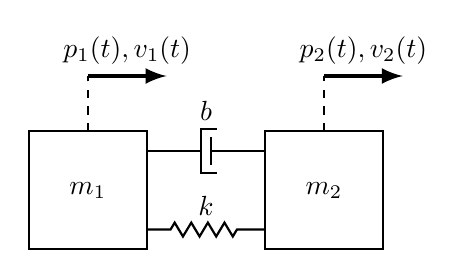
\begin{tikzpicture}
     \tikzstyle{spring}=[thick, decorate, decoration={zigzag, pre length=0.3cm, post length=0.3cm, segment length=6}]

     \tikzstyle{damper}=[thick,decoration={markings,
       mark connection node=dmp,
       mark=at position 0.5 with
       {
         \node (dmp) [thick,inner sep=0pt,transform shape,rotate=-90,minimum
     width=15pt,minimum height=3pt,draw=none] {};
         \draw [thick] ($(dmp.north east)+(2pt,0)$) -- (dmp.south east) -- (dmp.south
     west) -- ($(dmp.north west)+(2pt,0)$);
         \draw [thick] ($(dmp.north)+(0,-5pt)$) -- ($(dmp.north)+(0,5pt)$);
       }
     }, decorate]

     \tikzstyle{ground}=[fill,pattern=north east lines,draw=none,minimum
     width=0.75cm,minimum height=0.3cm]

     \node[draw,outer sep=0pt,thick] (M1) [minimum width=1.5cm, minimum height=1.5cm] {$m_1$};
     \node[draw,outer sep=0pt,thick] (M2) at (3,0) [minimum width=1.5cm, minimum height=1.5cm] {$m_2$};
     \draw[spring] ($(M1.east) - (0,0.5)$) -- ($(M2.west) - (0,0.5)$)
     node [midway, above = 0.05cm] {$k$};
     \draw[damper] ($(M1.east) + (0,0.5)$) -- ($(M2.west) + (0,0.5)$)
     node [midway, above = 0.25cm] {$b$};

     \draw[thick, dashed] ($(M1.north)$) -- ($(M1.north) + (0,0.7)$);
     \draw[thick, dashed] ($(M2.north)$) -- ($(M2.north) + (0,0.7)$);
     \draw[ultra thick, -latex] ($(M2.north) + (0,0.7)$) --
                                ($(M2.north) + (1,0.7)$)
                                node [midway, above] {$p_2(t), v_2(t)$};
     \draw[ultra thick, -latex] ($(M1.north) + (0,0.7)$) --
                                ($(M1.north) + (1,0.7)$)
                                node [midway, above] {$p_1(t), v_1(t)$};
   \end{tikzpicture}
 \end{document}
